% !TeX root = ../main.tex
\chapter{Applications of the differential calculus}

\lettrine{I}{n} the previous chapter we introduced various notions of differentials for higher dimensional functions (scalar fields, vector fields, paths, etc.).
In this chapter we now explore various applications of these notions and work with some of the implementations, rather than just the theory.
Firstly we will consider certain partial differential equations which we now have the tools to solve.
Then the majority of the chapter is devoted to searching for extrema (minima / maxima) in various different scenarios.
This extends what we already know for functions in \(\bR\) and we will find that in higher dimensions many more possibilities and subtleties exist.

\section{Partial differential equations}

There are a huge number of different types of partial differential equations and here we consider just two types \emph{first order linear PDEs} and the \emph{1D wave equation}.
We start by consider an example of the first type.

\begin{example*}
    Find all solutions of the partial differential equation
    \(3 \frac{\partial f}{\partial x}(x,y) + 2 \frac{\partial f}{\partial y} (x,y) = 0\).
\end{example*}

\begin{solution}
    The given PDE is equivalent to
    \(\left( \begin{smallmatrix}
            3 \\ 2
        \end{smallmatrix} \right)
    \cdot
    \nabla f(x,y) =0\).
    We can also phrase this in terms of the directional derivative, namely
    \[
        D_{v}f(x,y) = 0 \quad \text{where \(v=\left( \begin{smallmatrix}
                3 \\ 2
            \end{smallmatrix} \right)\)}.
    \]
    This means that if a function \(f\) is a solution to the PDE then it is constant in the direction \(\left( \begin{smallmatrix}
            3 \\ 2
        \end{smallmatrix} \right)\).
    This means that all solutions have the form \(f(x,y) = g(2x-3y)\) for some \(g:\bR \to \bR\).
\end{solution}

The same idea as above gives the following general result.

\begin{theorem}
    Let \(g:\bR\to\bR\) be differentiable, \(a,b\in \bR\), \((a,b)\neq (0,0)\).
    If \(f(x,y)= g(bx-ay)\) then
    \[
        a \frac{\partial f}{\partial x} (x,y) + b \frac{\partial f}{\partial y} (x,y) = 0.
    \]
    Conversely, every \(f\) which satisfies this equation is of the form \(g(bx-ay)\).
\end{theorem}

\begin{proof}
    First we prove \textbf{(\(\Rightarrow\))}.
    If \(f(x,y)= g(bx-ay)\) then, by the chain rule,
    \[
        \partial_x f(x,y) = bg'(bx-ay),
        \quad
        \partial_y f(x,y) = -ag'(bx-ay).
    \]
    Consequently \(a\partial_x f(x,y) + b \partial_y f(x,y) = a bg'(bx-ay) - abg'(bx-ay) = 0\).

    Now we prove \textbf{(\(\Leftarrow\))}.
    It's convenient to work in coordinates which correspond to the lines along which the solutions are constant.
    Let \(\left(\begin{smallmatrix}
            u\\ v
        \end{smallmatrix}\right)
    = \left(\begin{smallmatrix}
            a & b \\ b & -a
        \end{smallmatrix}\right)
    \left(\begin{smallmatrix}
            x \\ y
        \end{smallmatrix}\right)\).
    This means that
    \(\left(\begin{smallmatrix}
            x\\ y
        \end{smallmatrix}\right)
    = \frac{-1}{a^2 + b^2} \left(\begin{smallmatrix}
            a & b \\ b & -a
        \end{smallmatrix}\right)
    \left(\begin{smallmatrix}
            u \\ v
        \end{smallmatrix}\right)\).
    Let \(h(u,v)=f(\frac{au + bv}{a^2 + b^2}, \frac{bu-av}{a^2+b^2})\).
    Calculate
    \[
        \partial_u h(u,v)
        = \tfrac{1}{{a^2 + b^2}}
        \left( a \partial_x f
        + b \partial_y f \right)  (au + bv, bu-av) = 0.
    \]
    Namely, \(h(u,v)\) is a function of \(v\) only so take \(g(v) = h(u,v)\) and so \(f(x,y) = g(bx-ay)\).
\end{proof}

Now we look at another type of PDE.
The \emph{1D wave equation} is
\[
    \frac{\partial^2 f}{\partial x^2}(x,t) = c^2  \frac{\partial^2 f}{\partial t^2}(x,t).
\]
Here \(x\) represents the position along string,
\(t\) is time and \(f(x,t)\) is the displacement of the string from the centre at position \(x\), at time \(t\).
The constant \(c\) is a fixed parameter depending on the string.

This partial differential equation is derived from the equation of motion \(F = m a\) where \(F\) is the tension in the string, \(a\) is the acceleration from horizontal and \(m\) is the mass of a little piece of the string.
The equation is valid for small displacement.
In this case the \emph{boundary conditions} are natural: Are the ends of the string fixed? Is only one end fixed? At time \(t=0\), is the string already moving?

\begin{theorem}
    Let \(F\) be a twice differentiable function and \(G\) a differentiable function.

    \noindent
    \textbf{1.} The function defined as
    \begin{equation}
        \label{eq:wave}
        f(x,t) = \frac{1}{2}(F(x+ct) + F(x-ct)) + \frac{1}{2c} \int_{x-ct}^{x+ct} G(s) \ ds
    \end{equation}
    satisfies \(   \frac{\partial^2 f}{\partial x^2}(x,t) = c^2  \frac{\partial^2 f}{\partial t^2}(x,t) \),
    \(f(x,0) = F(x)\)
    and \(\frac{\partial f}{\partial t}(x,0) = G(x)\).

    \noindent
    \textbf{2.} Conversely, if a solution of  \(   \frac{\partial^2 f}{\partial x^2}(x,t) = c^2  \frac{\partial^2 f}{\partial t^2}(x,t) \) satisfies
    \[\frac{\partial^2 f}{\partial x \partial t}(x,t) = \frac{\partial^2 f}{\partial t \partial x}(x,t),\]
    then it has the above form \eqref{eq:wave}.
\end{theorem}


\begin{proof}[Proof of part 1.]
    Let \(f(x,t)\) be as defined \eqref{eq:wave} in the statement of the theorem.
    We calculate
    \[
        \begin{aligned}
            \tfrac{\partial f}{\partial x} (x,t)
             & = \tfrac{1}{2} \left(F'(x+ct) + F'(x-ct)\right)
            + \tfrac{1}{2c}\left(G(x+ct) - G(x-ct)\right)               \\
            \tfrac{\partial^2 f}{\partial x^2}(x,t)
             & = \tfrac{1}{2} \left(F''(x+ct) + F''(x-ct)\right)
            + \tfrac{1}{2c}\left(G'(x+ct) - G'(x-ct)\right)             \\
            \tfrac{\partial f}{\partial t} (x,t)
             & = \tfrac{1}{2} \left(cF'(x+ct) - c F'(x-ct)\right)
            + \tfrac{1}{2}\left(G(x+ct) + G(x-ct)\right)                \\
            \tfrac{\partial^2 f}{\partial t^2} f(x,t)
             & = \tfrac{1}{2} \left(c^2F''(x+ct) + c^2 F''(x-ct)\right)
            + \tfrac{c}{2}\left(G'(x+ct) + G'(x-ct)\right)
        \end{aligned}
    \]
    Observe that  \(   \frac{\partial^2 f}{\partial x^2}(x,t) = c^2  \frac{\partial^2 f}{\partial t^2}(x,t) \).
    Observe that \(f(x,0) = F(x)\)
    and \(\frac{\partial f}{\partial t}(x,0) = G(x)\).
\end{proof}

\begin{proof}[Proof of part 2.]
    Suppose that \(f\) satisfies the 1D wave equation;
    Introduce \(u = x + ct\), \(v=x-ct\)
    and observe that \(x = \frac{u+v}{2}\), \(t=\frac{u-v}{2c}\).
    Define \(g(u,v) = f(x,t) = f(   \frac{u+v}{2} , \frac{u-v}{2c} )\).
    By the chain rule
    \[
        \begin{aligned}
            \tfrac{\partial g}{\partial u}(u,v)
             & = \tfrac{1}{2} \tfrac{\partial f}{\partial x}(   \tfrac{u+v}{2} , \tfrac{u-v}{2c} )
            + \tfrac{1}{2c} \tfrac{\partial f}{\partial t}(   \tfrac{u+v}{2} , \tfrac{u-v}{2c} )                      \\
            \tfrac{\partial^2 g}{\partial v \partial u}(u,v)
             & = \tfrac{1}{4} \tfrac{\partial^2 f}{\partial x^2}(   \tfrac{u+v}{2} , \tfrac{u-v}{2c} )
            - \tfrac{1}{4c} \tfrac{\partial^2 f}{\partial x\partial t}(   \tfrac{u+v}{2} , \tfrac{u-v}{2c} )          \\
             & \ \ +  \tfrac{1}{4c} \tfrac{\partial^2 f}{\partial x \partial t}(   \tfrac{u+v}{2} , \tfrac{u-v}{2c} )
            -  \tfrac{1}{4c^2} \tfrac{\partial^2 f}{\partial t^2}(   \tfrac{u+v}{2} , \tfrac{u-v}{2c} ) = 0.
        \end{aligned}
    \]
    So \( \tfrac{\partial g}{\partial u}(u,v) = \varphi_0(u)\) and \(g(u,v) = \varphi_1(u) + \varphi_2(v)\).
    I.e., \(f(x,t) = \varphi_1(x+ct) + \varphi_2(x-ct)\).
    Let
    \[
        F(x) = \varphi_1(x) + \varphi_2(x).
    \]
    This means that
    \(F'(x) = \varphi_1'(x) + \varphi_2'(x)\)
    and \(\frac{\partial f}{\partial t}(x,t) = c\varphi_1(x+ct) - c\varphi_2(x-ct)\).
    Let
    \[
        G(x) = \frac{\partial f}{\partial t}(x,0) = c\varphi_1(x) - c\varphi_2(x). \qedhere
    \]
\end{proof}

\section{Extrema (minima / maxima / saddle)}

Let \(S\subset \bR^n\) be open,
\(f:S \to \bR\) be a scalar field
and \(\aa \in S\).

\begin{definition}[absolute min/max]
    If \(f(\aa)\leq f(\xx)\) (resp.\ \(f(\aa)\geq f(\xx)\)) for all \(\xx \in S\), then \(f(\aa)\) is said to be the \emph{absolute} minimum (resp.\ maximum) of \(f\).
\end{definition}

\begin{definition}[relative min/max]
    If \(f(\aa)\leq f(\xx)\) (resp.\ \(f(\aa)\geq f(\xx)\)) for all \(\xx \in B(\aa,r)\) for some \(r>0\), then \(f(\aa)\) is said to be a \emph{relative} minimum (resp.\ maximum) of \(f\).
\end{definition}

Collectively we call the these points the \emph{extrema} of the scalar field.
In the case of a scalar field defined on \(\bR^2\) we can visualize the scalar field as a 3D plot like Figure~\ref{fig:bumps}.
Here we see the extrema as the ``flat'' regions.
In this setting we use \emph{global} as a synonym of \emph{absolute} and \emph{local} as a synonym of \emph{relative}.


\begin{figure}[htb]
    \begin{center}
        \includegraphics{bumps.pdf}
        \caption{$f(x,y) := x e^{-(x^2y^2)}  + \frac{1}{4}e^{y^\frac{3}{10}}$}
        \label{fig:bumps}
    \end{center}
\end{figure}

To proceed it is convenient to connect the extrema with the behaviour of the gradient of the scalar field.

\begin{theorem}
    If \(f:S\to\bR\) is differentiable and has a relative minimum or maximum at \(\aa\), then \(\nabla f(\aa)=  \mathbf{0}\).
\end{theorem}

\begin{proof}
    Suppose \(f\) has a relative minimum at \(\aa\) (or consider \(-f\)).
    For any unit vector \(\vv\) let \(g(u) = f(\aa+u\vv)\).
    We know that \(g:\bR \to \bR\) has a relative minimum at \(u=0\) so \(u'(0)=0\).
    This means that the directional derivative \(D_{\vv} f(\aa) = 0\) for every \(\vv\).
    Consequently this means that \(\nabla f (\aa)= \mathbf{0}\).
\end{proof}

\begin{figure}[htb]
    \begin{center}
        \includegraphics[width=0.5\textwidth]{inflection.pdf}
        \caption{\(\nabla f(\aa) =  \mathbf{0}\) doesn't imply a minimum or maximum at \(\aa\) as seen for the function \(f(x):=x^3\).}
    \end{center}
\end{figure}

Observe that here and in the subsequent text, we can always consider the case of \(f:\bR \to \bR\), i.e., the case of \(\bR^n\) where \(n=1\).
Everything still holds and reduces to the arguments and formulae previously developed for functions of one variable.


\begin{definition}[stationary point]
    If \(\nabla f(\aa)=0\) then \(\aa\) is called a \emph{stationary point}.
\end{definition}


\begin{figure}[htb]
    \begin{center}
        \includegraphics[width=0.5\textwidth]{bowl.pdf}
        \caption{If \(f(x,y)=x^2+y^2\) then \(\nabla f(x,y) = \left(\begin{smallmatrix}
                2x\\2y
            \end{smallmatrix}\right)\) and \(\nabla f(0,0) =\left(\begin{smallmatrix}
                0\\0
            \end{smallmatrix}\right) \). The point \((0,0)\) is an absolute minimum for \(f\).}
    \end{center}
\end{figure}


\begin{definition}[saddle point]
    If \(\nabla f(\aa)=0\) and \(\aa\) is neither a minimum nor a maximum then \(\aa\) is said to be a \emph{saddle point}.
\end{definition}



\begin{figure}
    \begin{center}
        \includegraphics{pringle.pdf}
        \caption{If \(f(x,y)=x^2-y^2\) then \(\nabla f(x,y) = \left(\begin{smallmatrix}
                2x\\-2y
            \end{smallmatrix}\right)\) and \(\nabla f(0,0) =\left(\begin{smallmatrix}
                0\\0
            \end{smallmatrix}\right) \). The point \((0,0)\) is a saddle point for \(f\).}
    \end{center}
\end{figure}


\section{Hessian matrix}

To proceed it is useful to develop the idea of a second order Taylor expansion in this higher dimensional setting.
In particular this will allow us to identify the local behaviour close to stationary points.
The main object for doing this is the \emph{Hessian matrix}.

\begin{definition}[Hessian matrix]
    Let \(f:\bR^2 \to\bR\) be twice differentiable.
    We write this scalar field as \(f(x,y)\).
    The \emph{Hessian matrix} at \(\aa\in \bR^2\) is defined as
    \[
        \mathbf{H} f (\aa)= \begin{pmatrix}
            \dfrac{\partial^2 f}{\partial x^2} (\aa)
             & \dfrac{\partial^2 f}{\partial x\,\partial y} (\aa)
            \\[2.2ex]
            \dfrac{\partial^2 f}{\partial y\,\partial x} (\aa)
             & \dfrac{\partial^2 f}{\partial y^2}(\aa)
        \end{pmatrix}.
    \]
\end{definition}

Observe that the Hessian matrix \(\mathbf{H} f (\aa)\) is a symmetric matrix since we know that \(\frac{\partial^2 f}{\partial x\,\partial y} (\aa) = \frac{\partial^2 f}{\partial y\,\partial x} (\aa)\).
The Hessian matrix is defined analogously in any dimensions as follows.
Let \(f:\bR^n \to\bR\) be twice differentiable.
The \emph{Hessian matrix} at \(\aa\in \bR^n\) is defined as
\[
    \mathbf{H} f (\aa)= \begin{pmatrix}
        \dfrac{\partial^2 f}{\partial x_1^2} (\aa)
         & \dfrac{\partial^2 f}{\partial x_1\,\partial x_2} (\aa)
         & \cdots
         & \dfrac{\partial^2 f}{\partial x_1\,\partial x_n}(\aa)  \\[2.2ex]
        \dfrac{\partial^2 f}{\partial x_2\,\partial x_1} (\aa)
         & \dfrac{\partial^2 f}{\partial x_2^2}(\aa)
         & \cdots
         & \dfrac{\partial^2 f}{\partial x_2\,\partial x_n}(\aa)  \\[2.2ex]
        \vdots
         & \vdots
         & \ddots
         & \vdots                                                 \\[2.2ex]
        \dfrac{\partial^2 f}{\partial x_n\,\partial x_1} (\aa)
         & \dfrac{\partial^2 f}{\partial x_n\,\partial x_2} (\aa)
         & \cdots
         & \dfrac{\partial^2 f}{\partial x_n^2}(\aa)
    \end{pmatrix}.
\]

Observe that the Hessian matrix is a symmetric matrix in any dimension.


\begin{lemma*}
    If \(\vv= \left( \begin{smallmatrix}
            v_1\\ \vdots \\v_n
        \end{smallmatrix} \right)  \) then\footnote{The notation \(\vv^{\mathbf{t}}\) denotes the transpose of the vector \(\vv\).} \(\vv^{\mathbf{t}} \ \mathbf{H} f (\aa) \ \vv = \sum_{j,k=0}^{n}
    \partial_{j}\partial_{k}f(\aa)
    v_j v_k \in \bR\).
\end{lemma*}

\begin{proof}
    %We consider the \(\bR^2\) case. 
    % Let \(\vv= \left( \begin{smallmatrix}
    %         v_1\\ \vdots \\v_n
    %     \end{smallmatrix} \right)  \).
    For convenience we use the notation
    \(\partial_{j}\partial_{k}f(\aa) = \frac{\partial^2 f}{\partial x_j\,\partial x_k} (\aa)\).
    We calculate that
    \[
        \begin{aligned}
            \vv^{\mathbf{t}} \ \mathbf{H} f (\aa) \ \vv
             & =
            \begin{pmatrix}
                v_1 & \cdots & v_n
            \end{pmatrix}
            \begin{pmatrix}
                \partial_{1}\partial_{1}f(\aa) & \cdots &
                \partial_{1}\partial_{n}f(\aa)                   \\
                \vdots                         & \ddots & \vdots \\
                \partial_{n}\partial_{1}f(\aa) & \cdots &
                \partial_{n}\partial_{n}f(\aa)
            \end{pmatrix}
            \begin{pmatrix}
                v_1 \\ \vdots \\v_n
            \end{pmatrix}    \\
             & = \sum_{j,k=0}^{n}
            \partial_{j}\partial_{k}f(\aa)
            v_j v_k
        \end{aligned}
    \]
    as required.
\end{proof}


\begin{example*}
    Let \(f(x,y)=x^2-y^2\).
    The gradient and the Hessian are respectively
    \[
        \begin{aligned}
            \nabla f(x,y)      & =\begin{pmatrix}
                                      \frac{\partial f}{\partial x} (x,y) \\[2.2ex]
                                      \frac{\partial f}{\partial y} (x,y)
                                  \end{pmatrix} =   \begin{pmatrix}
                                                        2x \\-2y
                                                    \end{pmatrix},         \\
            \mathbf{H} f (x,y) & = \begin{pmatrix}
                                       \frac{\partial^2 f}{\partial x^2} (x,y)
                                        & \frac{\partial^2 f}{\partial x\,\partial y} (x,y)
                                       \\[2.2ex]
                                       \frac{\partial^2 f}{\partial y\,\partial x} (x,y)
                                        & \frac{\partial^2 f}{\partial y^2}(x,y)
                                   \end{pmatrix}
            = \begin{pmatrix}
                  2
                   & 0
                  \\[2.2ex]
                  0
                   & -2
              \end{pmatrix}.
        \end{aligned}
    \]
    The point \((0,0)\) is a stationary point since \(\nabla f(0,0) =\left(\begin{smallmatrix}
            0\\0
        \end{smallmatrix}\right) \).
\end{example*}


\subsubsection*{Second order Taylor formula for scalar fields}

First let's recall the first order Taylor approximation from Theorem~\ref{thm:differential}.
If \(f\) is differentiable at \(\aa\)
then
\(  f(\aa+  \vv) = f(\aa)  + \nabla f(\aa) \cdot \vv + \epsilon(\vv)\).
If \(\aa\) is a stationary point then this only tells us that \(  f(\aa+  \vv) = f(\aa)  +  \epsilon(\vv)\) so a natural next question is to search for slightly more detailed information.

\begin{theorem}[second order Taylor]
    Let \(f\) be a scalar field twice differentiable on \(B(\aa,r)\).
    Then, if \(\norm{\vv}\leq r\),
    \[
        f(\aa+\vv) \approx f(\aa) + \nabla f(\aa) \cdot \vv + \frac{1}{2} \vv^{\mathbf{t}} \ \mathbf{H} f (\aa) \ \vv
    \]
    in the sense that the error is \(\littleo{\norm{\vv}^2}\).
\end{theorem}




\begin{proof}[Proof of second order Taylor formula]
    Let \(g(u) = f(\aa + u \vv)\).
    The Taylor expansion of \(g\) tells us that
    \(g(1) = g(0) + g'(0) + \frac{1}{2} g''(c)\) for some \(c\in (0,1)\).
    Since \(g(u) = f(a_1 + uv_1, \ldots, a_n + u v_n)\), by the chain rule,
    \[
        g'(u) = \sum_{j=1}^{n} \partial_j f( a_1 + uv_1, \ldots, a_n + u v_n ) v_j
        =\nabla f( \aa + u \vv) \cdot \vv.
    \]
    Similarly
    \[
        g''(u) = \sum_{j,k=1}^{n} \partial_j\partial_k f( a_1 + uv_1, \ldots, a_n + u v_n ) v_j v_k
        =  \vv^{\mathbf{t}} \ \mathbf{H} f (\aa + u \vv) \ \vv.
    \]
    Consequently
    \(
    f(\aa+\vv) = f(\aa) + \nabla f(\aa) \cdot \vv + \frac{1}{2} \vv^{\mathbf{t}} \ \mathbf{H} f (\aa + c\vv) \ \vv
    \).
    We define the ``error'' in the approximation as \(\epsilon(\vv) = \frac{1}{2} \frac{1}{\norm{\vv}^2} \vv^{\mathbf{t}} (\mathbf{H} f (\aa + c\vv) - \mathbf{H} f (\aa)  ) \vv\)
    and estimate that
    \[
        \abs{\epsilon(\vv)} \leq \sum_{j,k=0}^{n}
        \frac{v_j v_k}{\norm{\vv}^2} \left( \partial_{j}\partial_{k}f(\aa+c\vv)-\partial_{j}\partial_{k}f(\aa) \right).
    \]
\end{proof}


\section{Classifying stationary points}

In order to classify the stationary points we will take advantage of the Hessian matrix and therefore we need to first understand the follow fact about real symmetric matrices.

\begin{theorem}
    Let \(A\) be a real symmetric matrix and let
    \(Q(\vv) =  \vv^{\mathbf{t}} A  \vv  \).
    Then
    \begin{itemize}
        \item \(Q(\vv) > 0\) for all \(\vv \neq \mathbf{0}\) if and only if all eigenvalues of \(A\) are positive;
        \item \(Q(\vv) < 0\) for all \(\vv \neq \mathbf{0}\) if and only if all eigenvalues of \(A\) are negative.
    \end{itemize}
\end{theorem}

\begin{proof}
    Since \(A\) is symmetric it can be diagonalised by  matrix \(B\)  which is orthogonal (\(B^{\mathbf{t}}=B^{-1}\))
    \[
        D = B^{\mathbf{t}} A B =
        \begin{pmatrix}
            \lambda_1 & \cdots & 0         \\
            \vdots    & \ddots & \vdots    \\
            0         & \cdots & \lambda_n
        \end{pmatrix}.
    \]
    This means that
    \[
        Q(\vv) = \vv^{\mathbf{t}} B^{\mathbf{t}} B A B^{\mathbf{t}} B \vv  = \ww^{\mathbf{t}} D \ww = \sum_{j} \lambda_j w_j^2
    \]
    where \(\ww = B \vv\).
    Observe that, if all \(\lambda_j >0\) then \( \sum_{j} \lambda_j w_j^2  >0\).

    In order to prove the other direction in the ``if and only if'' statement, observe that \(Q(B \uu_k ) = \lambda_k\). This means that, if \(Q(\vv) > 0\) for all \(\vv \neq \mathbf{0}\) then \(\lambda_k>0\) for all \(k\).
\end{proof}

\begin{theorem}[classification of stationary points]
    Let \(f\) be a scalar field twice differentiable on \(B(\aa,r)\).
    Suppose  \(\nabla f(\aa) = \mathbf{0}\).
    Then
    \begin{itemize}
        \item \emph{All} eigenvalues of \(\mathbf{H} f (\aa)\) are positive then \(f\) has a relative minimum at \(\aa\);
        \item \emph{All} eigenvalues of \(\mathbf{H} f (\aa)\) are negative then \(f\) has a relative maximum at \(\aa\);
        \item Some eigenvalues positive and some negative then \(\aa\) is a saddle point.
    \end{itemize}
\end{theorem}

\begin{proof}
    Let \(Q(\vv) =  \vv^{\mathbf{t}} \mathbf{H} f (\aa) \vv  \),  \(\ww = B \vv\) and let \(\Lambda := \min_j \lambda_j\).
    Observe that \(\norm{\ww} =  \norm{\vv}\) and that \(Q(\vv)=  \sum_{j} \lambda_j w_j^2  \geq \Lambda \sum_{j} w_j^2 = \Lambda  \norm{\vv}^2 \).
    We have them 2\textsuperscript{nd}-order Taylor
    \[
        f(\aa+\vv) - f(\aa)
        =  \frac{1}{2} \vv^{\mathbf{t}} \ \mathbf{H} f (\aa) \ \vv + \norm{\vv}^2 E_2(\aa,\vv)
        \geq  \left(\tfrac{\Lambda}{2} - E_2(\aa,\vv) \right) \norm{\vv}^2;
    \]
    Since \(E_2(\aa,\vv) \to 0\) as \(\norm{\vv}\to 0\), \(\abs{E_2(\aa,\vv)} < \tfrac{\Lambda}{2}\) when \(\norm{\vv}\) is small.

    Analogous argument for the second part. For final part consider \(\vv_j\) which is eigenvector for \(\lambda_j\) and apply the argument of first or second part.
\end{proof}

\section{Attaining extreme values}

Here we explore the extreme value theorem for continuous scalar fields.
The argument will be in two parts:
Firstly we show that continuity implies boundedness;
Secondly we show that boundedness implies that the maximum and minimum are attained.
We use the following notation for \emph{intervals} / \emph{rectangles} / \emph{cuboids}, etc.
If \(\aa = (a_1,\ldots,a_n)\) and  \(\bb = (b_1,\ldots,b_n)\)
then we consider the \(n\)-dimensional closed Cartesian product
\[
    [\aa,\bb] = [a_1,b_1] \times \cdots \times [a_n,b_n].
\]
We call this set a \emph{rectangle} (independent of the dimension).
As a first step it is convenient to know that all sequences in our setting have convergent subsequences.

\begin{theorem}[Bolzano–Weierstrass]
    If \({\{\xx_{n}\}}_{n}\) is a sequence in \( [\aa,\bb]\)
    there exists a convergent subsequence \({\{\xx_{n_j}\}}_{j}\).
\end{theorem}

\begin{proof}
    In order to prove the theorem we construct the subsequence.
    Firstly we divide \( [\aa,\bb]\) into sub-rectangles of size half the original.
    We then choose a sub-rectangle which contains infinite elements of the sequence and choose the first of these elements to be part of the sub-sequence.
    We repeat this process by again dividing the sub-rectangle we chose by half and choosing the next element of the subsequence.
    We repeat to give the full subsequence.
\end{proof}

\begin{theorem}[boundedness of continuous scalar fields]
    Suppose that \(f\) is a scalar field continuous at every point in the closed rectangle \([\aa,\bb]\).
    Then \(f\) is bounded on \([\aa,\bb]\) in the sense that there exists \(C>0\) such that \(\abs{f(\xx)} \leq C\) for all \(\xx \in [\aa,\bb]\).
\end{theorem}

\begin{proof}
    Suppose the contrary: for all \(n\in\bN\) there exists \(\xx_n\in [\aa,\bb]\) such that \(\abs{f(\xx_n)}>n\).
    \href{https://en.wikipedia.org/wiki/Bolzano%E2%80%93Weierstrass_theorem}{Bolzano–Weierstrass} theorem means that there exists a subsequence \({\{\xx_{n_j}\}}_{j}\) converges to \( \xx \in [\aa,\bb]\).
    Continuity of \(f\) means that \(f(\xx_{n_j})\) converges to \(f(\xx)\). This is a contradiction and hence the theorem is proved.
\end{proof}


We can now use the above result on the boundedness in order to show that the  extreme values are actually obtained.

\begin{theorem}[extreme value theorem]
    Suppose that \(f\) is a scalar field continuous at every point in the closed rectangle \([\aa,\bb]\).
    There there exist points \( \xx, \yy \in [\aa,\bb]\) such that
    \[
        f(\xx) = \inf f
        \quad \text{and} \quad
        f(\yy)= \sup f.
    \]
\end{theorem}

\begin{proof}
    By the boundedness theorem \(\sup f\) is finite and so there exists a sequence  \({\{\xx_{n}\}}_{n}\)  such that \(f(\xx_n)\) converges to \(\sup f\).
    Bolzano–Weierstrass theorem implies that there exists a subsequence  \({\{\xx_{n_j}\}}_{j}\) which converges to \( \xx \in [\aa,\bb]\).
    By continuity \(f(\xx_n) \to f(\xx) = \sup f\).
\end{proof}




\section{Extrema with constraints (Lagrange multipliers)}

We now consider a slightly different problem to the one earlier in this chapter.
There we wished to find the extrema of a given scalar field.
Here the general problem is to minimise or maximise a given scalar field \(f(x,y)\) under the constraint \(g(x,y) = 0\).
Subsequently we will also consider the same problem but in higher dimensions.
We can visualize this problem as shown in Figure~\ref{fig:lagrange}.
For this graphic representation we draw the constraint and also various level sets of the function that we want to find the extrema of.
The graphical representation suggests to us that at the ``touching point'' the gradient vectors are parallel.
In other words, \(\nabla f = \lambda \nabla g\) for some \(\lambda \in \bR\).
The implementation of this idea is the \href{https://en.wikipedia.org/wiki/Lagrange_multiplier}{method of Lagrange multipliers}.


\begin{theorem}[Lagrange multipliers]
    Suppose that a differentiable scalar field \(f(x,y)\) has a relative minimum or maximum when it is subject to the constraint
    \[
        g(x,y) = 0.
    \]
    Then there exists a scalar \(\lambda\) such that, at the extremum point,
    \[
        \nabla f = \lambda \nabla g.
    \]
\end{theorem}
In higher dimensions, with additional constraints
\begin{theorem*}[Lagrange multipliers]
    Suppose that a differentiable scalar field \(f(x_1,\ldots,x_n)\) has a relative minimum or maximum when it is subject to \(m\) constraints
    \[
        g_1(x_1,\ldots,x_n) = 0,
        \dots , g_m(x_1,\ldots,x_n)=0,
    \]
    where \(m<n\), and that the \(\nabla g_k\) are all linearly independent.
    Then there exist \(m\) scalars \(\lambda_1,\ldots,\lambda_m\) such that
    \[
        \nabla f = \lambda_1 \nabla g_1 + \cdots + \lambda_m \nabla g_m
    \]
    at the extremum point.
\end{theorem*}

\begin{figure}[htb]
    \begin{center}
        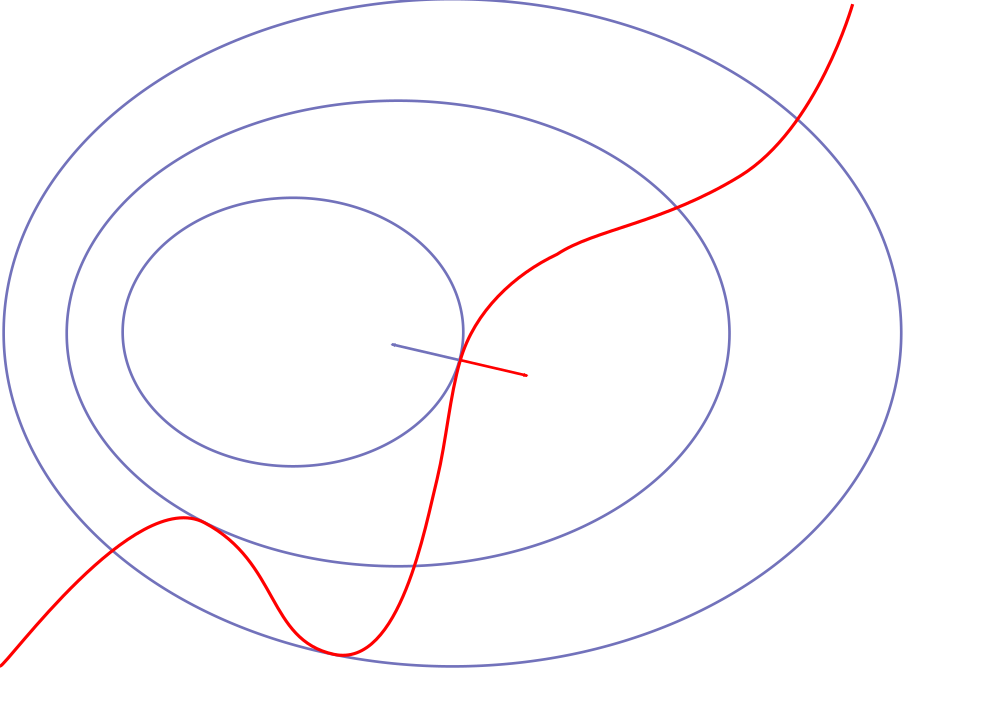
\includegraphics{lagrange.pdf}
        \caption{Searching for the extrema of \(f\) under constraint \(g(x,y)=0\)}
        \label{fig:lagrange}
    \end{center}
\end{figure}




